% !TeX program = xelatex
% =====================================================================
% 2023 高教社杯全国大学生数学建模竞赛 C 题
% 蔬菜类商品的自动定价与补货决策
% ---------------------------------------------------------------------
% 编译方式：xelatex main.tex，连续编译两遍（交叉引用第二遍才齐）
% 图片说明：figs/ 下 fig1.png ~ fig9.png 与正文图 1~9 一一对应，
%           原始高清图见 仓库内 问题1-SKU全息画像与关联分析/figs/
% 分工说明：本文当前只完成问题 1（第 5 节与摘要对应段）；
%           问题 2、3、4 的章节与摘要句留空，位置均用 % TODO 标出
% 写作规范：deAiWriting（三判据：可替换性 / 数值密度 / 决策痕迹）
% =====================================================================
\documentclass[zihao=-4,a4paper]{ctexart}
\usepackage[margin=2.5cm]{geometry}
\usepackage{amsmath,amssymb}
\usepackage{graphicx}
\usepackage{booktabs}
\usepackage{caption}
\usepackage{float}
\graphicspath{{figs/}}
\captionsetup{font=small,labelfont=bf,skip=6pt}
\linespread{1.4}
\setlength{\parskip}{0.35em}

\begin{document}

% ------------------------------ 摘要页 ------------------------------
\begin{center}
{\zihao{3}\textbf{基于SKU全息画像与相关性归因的蔬菜类商品\\销售分布规律与相互关系分析}}
\end{center}

\vspace{0.8em}
\begin{center}\textbf{摘\quad 要}\end{center}

蔬菜商品保鲜期短、单品长尾悬殊，摸清销售量的分布规律与相互关系是补货和定价的前提。本文以某商超 2020 年 7 月至 2023 年 6 月共 1,095 天、878,503 条销售流水为对象，先按 $C=P/(1-r)$ 把损耗率折入成本，再对 246 个有销售单品建立全息画像。

针对问题 1，分布规律层面：ABC 分析给出 28 个 A 类单品贡献销售额 69.27\%；波动度量改按周聚合，变异系数中位数由日粒度的 1.470 降至 0.691；熵权-TOPSIS 四梯队里 24 个热销单品以 9.8\% 的品种数贡献 47.42\% 的销量与 46.35\% 的毛利，得分与总销量的 Spearman 相关 0.527，分层并非按销量排队；Syntetos-Boylan 分类给出 42.3\% 的 Lumpy 单品，仅 13.8\% 适合标准预测模型。相互关系层面：三层归因显示品类日相关主要由月度共同波动决定（回归 $r=0.981$），去季节后 15 个品类对平均相关由 0.473 升至 0.523，茄类由 0.074$\sim$0.257 恢复至 0.30$\sim$0.40，茄类需求独立是季节相位制造的假象；共现网络以 lift 不低于 1.35 建边，分出 3 个跨品类社团，模块度 0.3983；36 组同款不同规格单品中 23 组 lift 小于 1 属替代关系，菌菇袋装与盒装 lift 达 2.18$\sim$4.52 属互补关系。最后按日毛利产出贪心选出 30 个单品，覆盖总销量 60.6\% 与总毛利 63.3\%，可作为问题 3 的初始解。

% TODO（队友补写）问题 2 摘要句：品类销售总量与成本加成定价的关系模型，
%                  以及 2023 年 7 月 1--7 日的日补货总量与定价策略结论
% TODO（队友补写）问题 3 摘要句：27~33 个单品的选品与补货定价结论
% TODO（队友补写）问题 4 摘要句：数据采集建议

稳健性方面，季节聚类在 $k=3,4,5$ 三档试算后取 5，簇内曲线峰值一致；成本修正使 8 个亏损单品显形，其中洪山菜薹莲藕拼装礼盒单位毛利 $-124.73$ 元/kg，不修正会被当成正常盈利品。

\vspace{0.6em}
\noindent\textbf{关键词：}\quad 蔬菜销售；ABC-XYZ 分层；熵权-TOPSIS；Syntetos-Boylan 分类；共现网络；相关性归因

\newpage

% ------------------------------ 正文 ------------------------------
\section{问题重述}

\subsection{问题背景}

生鲜商超里蔬菜类商品保鲜期短，品相随销售时间增加而变差，大部分品种当日未售出，隔日就无法再售，商超通常按天补货。蔬菜的进货交易时间通常在凌晨 3:00 至 4:00，商家须在不确切知道具体单品和进货价格的情况下，做出当日各品类的补货决策；定价一般采用成本加成方法，对运损和品相变差的商品打折销售。补货多少、定价多高，都取决于对市场需求的判断准不准。从需求侧看，蔬菜销售量与时间往往存在关联；从供给侧看，供应品种在 4 月至 10 月较为丰富，销售空间有限，合理的销售组合变得极为重要。附件 1 给出 6 个蔬菜品类的商品信息，附件 2 与附件 3 分别给出 2020 年 7 月 1 日至 2023 年 6 月 30 日的销售流水与批发价格，附件 4 给出各单品近期损耗率。

\subsection{待解决的问题}

题目要求依据附件建立数学模型解决四个问题。问题 1：蔬菜类商品不同品类或不同单品之间可能存在一定的关联关系，要求分析蔬菜各品类及单品销售量的分布规律及相互关系。问题 2：考虑商超以品类为单位做补货计划，要求分析各品类的销售总量与成本加成定价的关系，给出 2023 年 7 月 1 日至 7 日各品类的日补货总量与定价策略，使商超收益最大。问题 3：要求在可售单品总数控制在 27$\sim$33 个、各单品订购量满足最小陈列量 2.5 千克的约束下，根据 2023 年 6 月 24 日至 30 日的可售品种，给出 7 月 1 日的单品补货量与定价策略。问题 4：讨论商超还需采集哪些数据，这些数据对解决上述问题有何帮助。

% 本文件当前只完成问题 1；问题 2、3、4 由队友补写。

\section{问题分析}

问题 1 要同时回答两件事，分布规律与相互关系，两件事的分析路径不同，拆开处理。

分布规律这边先排三个坑。第一个坑是成本口径，附件 3 的批发价按天合并成面板后缺失 79.6\%，损耗率若不折算，品类毛利率整体虚高 7.7\%$\sim$16.5\%，利润侧的一切结论都会失真，所以先修成本再谈毛利。第二个坑是数据稀疏，246 个单品铺在 1,095 天上，零销售日大量存在，日粒度的波动指标会失真，分层前先做粒度试验。第三个坑是单一指标定层，只按销量排队得到的不是分层而是排序，本文用四套互补的分层各自回答一个问题，ABC-XYZ 回答库存策略，熵权-TOPSIS 回答单品梯队，Syntetos-Boylan 分类回答预测模型选型，量-利四象限回答毛利职责，四套结果相互印证。

相互关系这边分两条线。时间维度的共变用相关系数度量，但表面相关可能由季节相位制造，夏菜与冬菜旺季相反，负的季节项会盖住真实的日内联动，所以做三层归因把月度波动、季节指纹、日内联动分开；同日共现的关联用共现网络与归一化互信息度量，替代与互补关系在同款不同规格单品内部检验。附件 2 是天粒度流水而非小票，共现只能做到同日出现，这层信息边界在方法选型时已经计入。

% TODO（队友补写）问题 2 分析
% TODO（队友补写）问题 3 分析
% TODO（队友补写）问题 4 分析

\section{模型假设}

\begin{enumerate}
  \item \textbf{批发价月内平稳假设}：附件 3 批发价按天合并后缺失率 79.6\%，假设单品批发价在月内的变动远小于品类间差异，可用单品中位数配合前后向填充补齐面板，补齐后流水与批发价匹配率 100.00\%。目的：让成本口径覆盖全部流水，避免删除缺失期损失大半销售样本。
  \item \textbf{有效成本折算假设}：每售出 1 kg 陈列品需购入 $1/(1-r)$ kg，损耗率 $r$ 取附件 4 数值，六个品类在 7.12\%$\sim$14.14\% 之间；不考虑运输损耗、库存周转变质等附件未给出的损耗来源。目的：修正被系统性低估的成本。
  \item \textbf{退货非需求假设}：退货流水不代表真实需求，清洗时整体剔除，且不对退货当日需求做插值。目的：让销量序列反映真实需求。
  \item \textbf{退市判定假设}：近 180 天无销售的单品视为已退市，不进入候选池。目的：保证涉及选品的建议可执行。
  \item \textbf{周聚合波动假设}：单品需求波动以周销量变异系数度量，以 0.5 与 1.0 为界分三档；不用日粒度变异系数，零销售日使全体中位数达到 1.470，周聚合降到 0.691。目的：让波动分层可分辨。
  \item \textbf{样本期外推假设}：2020 年 7 月至 2023 年 6 月的结构规律对 2023 年下半年外推有效，不考虑供应结构性突变重现。目的：为后续补货与定价预测提供前提。
\end{enumerate}

对两条关键假设做设计说明。若不做假设 2，直接以批发价计成本，品类毛利率整体抬高 7.7\%$\sim$16.5\%，量-利四象限里利润品与问题品的分界整体右移，洪山菜薹两件深亏单品会被当成正常盈利品，后续定价建议的方向整个反掉。若不做假设 4，候选池会混入 110 个已退市单品、占销量 10.2\%，为它们给出的补货建议无法执行，选品问题的解空间被虚假放大。

\section{符号说明}

\begin{table}[H]
\centering
\caption{主要符号与含义}
\begin{tabular}{clc}
\toprule
符号 & 含义 & 单位 \\
\midrule
$P$ & 单品批发价 & 元/kg \\
$r$ & 单品损耗率 & 无量纲 \\
$C$ & 单位有效成本 & 元/kg \\
$m$ & 单位毛利（售价减有效成本） & 元/kg \\
$\mathrm{CV}$ & 变异系数（标准差除以均值） & 无量纲 \\
$\mathrm{ADI}$ & 平均需求间隔 & 天 \\
$w_j$ & 熵权法第 $j$ 维权重 & 无量纲 \\
$C_i$ & TOPSIS 贴近度 & 无量纲 \\
$\mathrm{lift}_{AB}$ & 单品 $A$、$B$ 的共现提升度 & 无量纲 \\
$\mathrm{NMI}$ & 归一化互信息 & 无量纲 \\
$Q$ & 共现网络模块度 & 无量纲 \\
$\rho$ & Spearman 秩相关系数 & 无量纲 \\
$E$ & 日毛利产出 & 元/天 \\
\bottomrule
\end{tabular}
\end{table}

\section{问题1模型的建立与求解}

\subsection{数据预处理与有效成本修正}

先算成本账。附件 3 的批发价只有 55,982 条记录，按天合并成 1,095 天乘 251 个单品的面板后，缺失 218,863 格，缺失率 79.6\%。对此有两条路，一是把缺失期的销售流水整段删掉，二是用单品批发价中位数配合前后向填充补齐。前一条路走不通，删掉 79.6\% 的日期等于把销售样本砍掉大半，分布规律的分析对象都没了；批发价月内变动很小，填充引入的误差远小于删样本的损失，故取后者，补齐后流水与批发价的匹配率 100.00\%。

清洗阶段剔除退货与明显异常记录，剩 878,503 条流水，251 个单品中 246 个有实际销售，归并为 6 个品类。成本口径不修正，后面的毛利分析会整体失真：每售出 1 kg 陈列品，进货端实际要准备 $1/(1-r)$ kg，其中 $r$ 是附件 4 给的损耗率，六个品类在 7.12\%$\sim$14.14\% 之间。由此建立有效成本模型
\begin{equation}
C = \frac{P}{1-r},
\end{equation}
式中 $P$ 为批发价。直接拿批发价当成本，毛利率会被整体抬高 7.7\%$\sim$16.5\%。修正后 246 个单品的毛利率中位数 33.1\%，单位毛利中位数 2.246 元/kg，单位毛利为负的有 8 个单品，亏损最深的洪山菜薹莲藕拼装礼盒达到 $-124.73$ 元/kg，这批单品后面还要单独说。

\subsection{品类的量价本利结构}

把六个品类的销量、销售额、毛利各自占比排在一起，错位立刻显形，结构见表 \ref{tab:category}。花叶类 99 个单品占销量 42.15\%，是门店的基本盘，销售额占比却只有 32.02\%，用销售额占比除以销量占比得到相对价格指数 0.76，六品类最低；花菜类反过来，指数 1.26 最高。

\begin{table}[H]
\centering
\caption{六品类的量价本利结构}
\label{tab:category}
\begin{tabular}{lrrrrrr}
\toprule
品类 & 单品数 & 销量占比/\% & 销售额占比/\% & 毛利占比/\% & 整体毛利率/\% & 平均损耗率/\% \\
\midrule
花叶类 & 99 & 42.15 & 32.02 & 33.51 & 31.18 & 10.28 \\
辣椒类 & 43 & 19.45 & 22.38 & 23.74 & 31.60 & 8.49 \\
食用菌 & 71 & 16.16 & 18.39 & 18.37 & 29.77 & 8.08 \\
花菜类 & 5 & 8.87 & 11.15 & 10.16 & 27.16 & 14.14 \\
水生根茎类 & 18 & 8.62 & 10.39 & 8.14 & 23.34 & 11.79 \\
茄类 & 10 & 4.76 & 5.67 & 6.08 & 31.95 & 7.12 \\
\bottomrule
\end{tabular}
\end{table}

直觉上均价最低的品类应该最不赚钱，账不是这么算的，花叶类毛利率 31.18\%，与茄类的 31.95\%、辣椒类的 31.60\% 同处第一梯队，反而高出花菜类的 27.16\% 与水生根茎类的 23.34\%。用毛利占比减销售额占比来度量错位，花叶类 $+1.49$ 个百分点，辣椒类 $+1.36$ 个百分点，水生根茎类 $-2.25$ 个百分点，见图 \ref{fig:misalign}。错位的原因要到成本端找，花叶类损耗率 10.28\%，明显低于花菜类的 14.14\% 与水生根茎类的 11.79\%，低价换来高周转与低损耗。单品层面差距更大，小米椒单位毛利 9.99 元/kg，大白菜 0.49 元/kg，差 20.5 倍。

\begin{figure}[H]
\centering
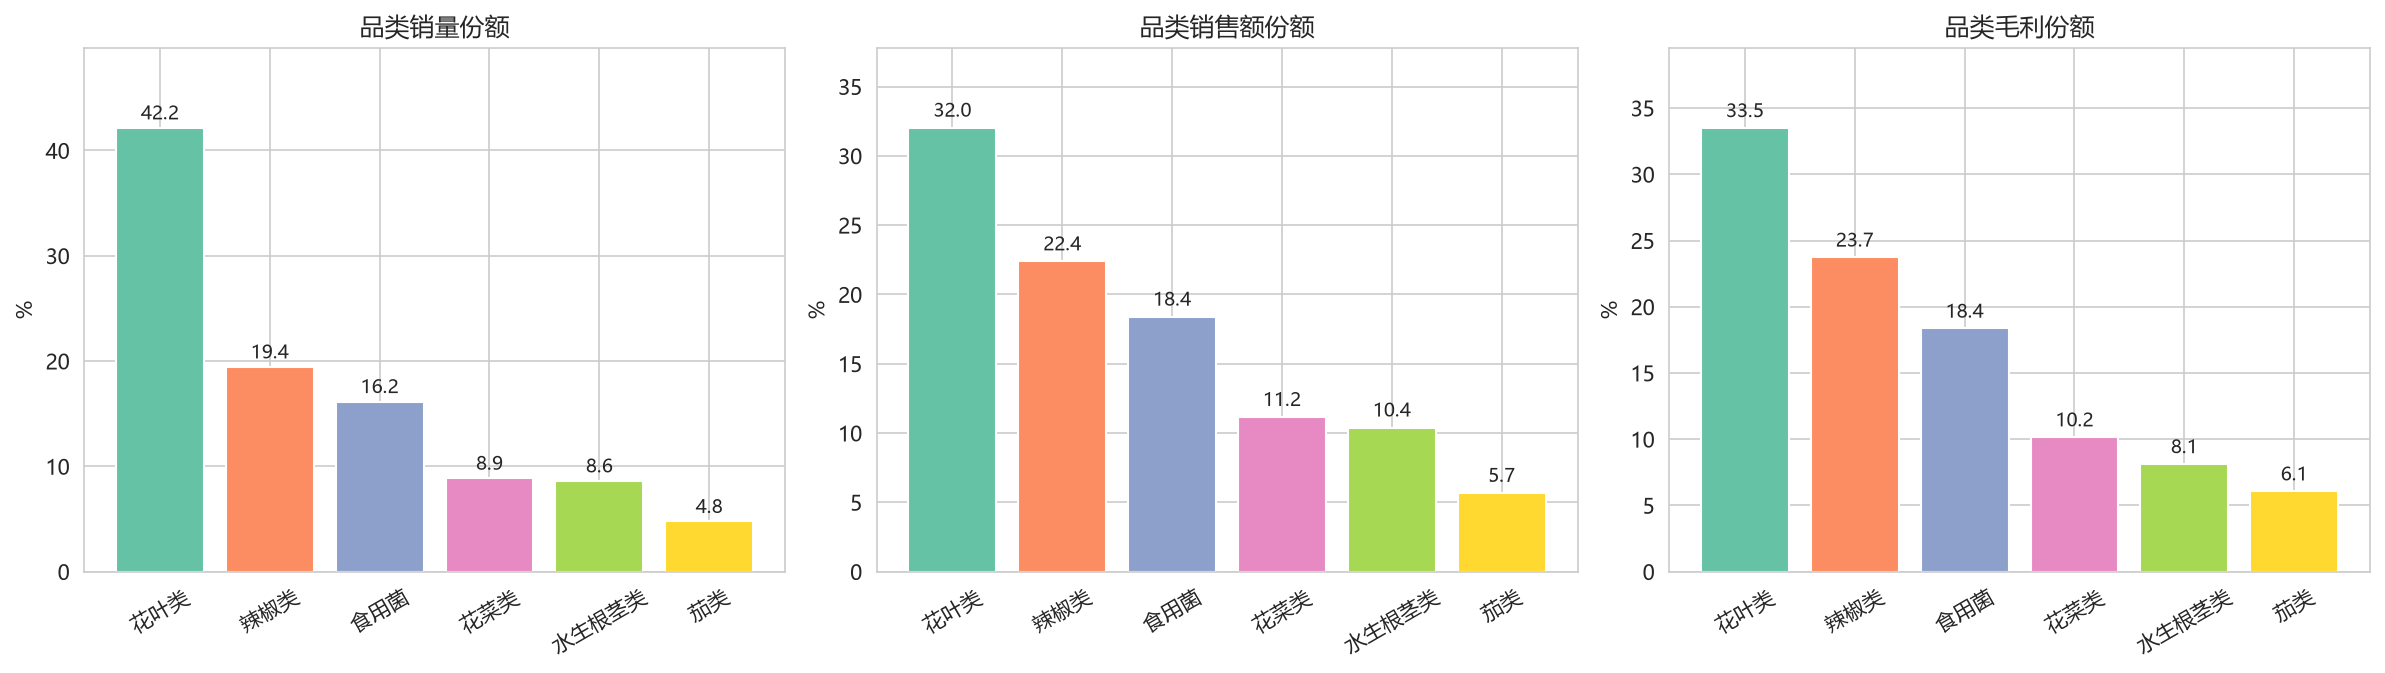
\includegraphics[width=0.92\textwidth]{fig1.png}
\caption{六品类销量、销售额、毛利三者占比的错位}
\label{fig:misalign}
\end{figure}

\subsection{ABC-XYZ 九宫格分层}

分层的第一个决定是换掉日粒度波动。ABC 按销售额累计 70\%、90\%、100\% 切分，得 A 类 28 个、B 类 35 个、C 类 183 个，销售额占比 69.27\%、20.54\%、10.19\%，头重脚轻的长尾结构一目了然。波动维度最初按日粒度算变异系数，结果全体日 CV 中位数 1.470，蔬菜单品并不是天天有人买，大量零销售日把 CV 抬得离谱，照这个标准切几乎全落进高波动档。改按周聚合，CV 中位数降到 0.691，以 0.5 与 1.0 为界得 X 类 35 个、Y 类 148 个、Z 类 63 个，三类动销率均值分别为 0.583、0.430、0.594。

两维交叉成九宫格，AX 5 个、AY 21 个、AZ 2 个、BX 4 个、BY 31 个、CX 26 个、CY 96 个、CZ 61 个，BZ 为空。格子一填出来，策略自己浮出来了：AX 与 AY 合计 26 个单品贡献 65.79\% 的销售额，前者波动小，可以签长期供货协议定量补货，后者要提高安全库存动态补；A 类里只有 2 个单品波动剧烈，留柔性补货的口子；CZ 的 61 个单品合计只贡献 1.77\% 销售额，属于末位淘汰与旺季临时上架的对象。图 \ref{fig:abcxyz} 把九宫格与各格策略放到一张图里。

\begin{figure}[H]
\centering
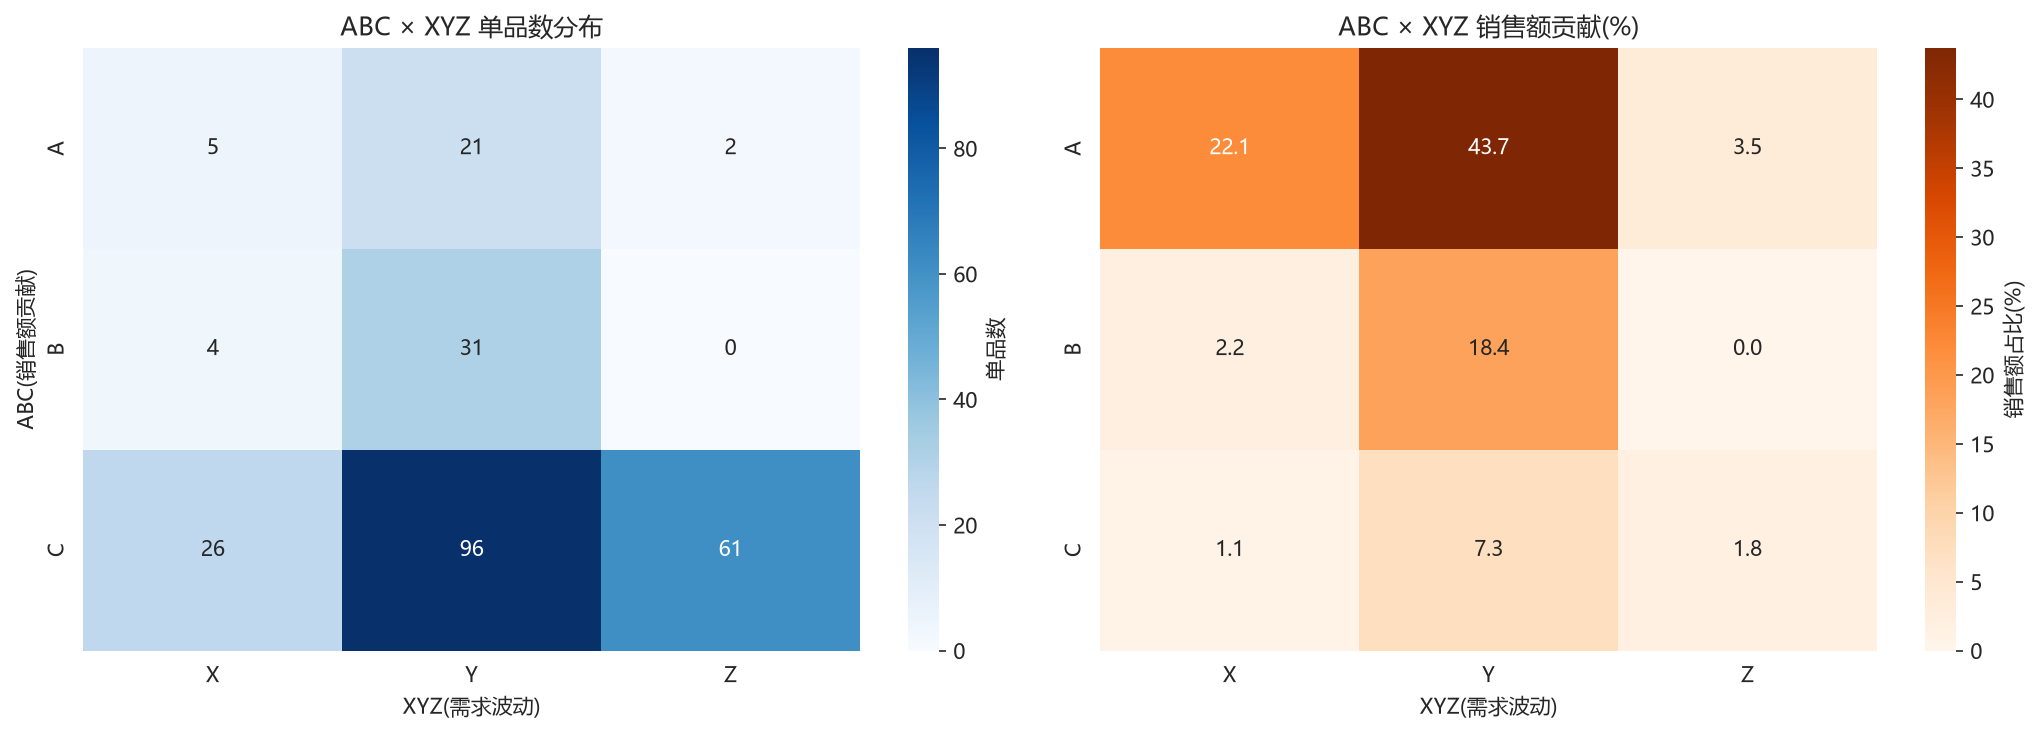
\includegraphics[width=0.92\textwidth]{fig2.png}
\caption{ABC-XYZ 二维分层矩阵与单元格策略}
\label{fig:abcxyz}
\end{figure}

\subsection{熵权-TOPSIS 四梯队}

我们最初打算对总销量、单日最大销量、日均销量做 KMeans 聚类，试算后发现三个特征高度共线，簇边界实际由规模一维决定，簇心也读不出业务含义，聚类在这里空转，弃掉。改走打分路线，四个维度分工：规模用总销量，广度用动销率即有售天数占比，强度用有售日日均销量，稳定用 $1/\mathrm{CV}$。规模与强度相关 0.807，广度与稳定相关 0.796，两组高相关分别来自销量水平与销售覆盖两个侧面，保留它们是为了把卖得多与常年有售分开计分。权重交给熵权法按信息量分配，对归一化后的特征矩阵
\begin{equation}
e_j=-\frac{1}{\ln n}\sum_{i=1}^{n}p_{ij}\ln p_{ij},\qquad
w_j=\frac{1-e_j}{\sum_{j=1}^{4}\left(1-e_j\right)},
\end{equation}
算得广度 0.2928 最高，稳定 0.2581 次之，强度 0.2403，规模 0.2089 最低。再以理想解贴近度排梯队，
\begin{equation}
C_i=\frac{D_i^{-}}{D_i^{+}+D_i^{-}},\qquad
D_i^{\pm}=\sqrt{\sum\nolimits_{j}\left(v_{ij}-v_j^{\pm}\right)^{2}},
\end{equation}
式中 $v_{ij}$ 为加权归一化矩阵元素，$v_j^{\pm}$ 为正负理想解分量。

TOPSIS 得分按 10\%、20\%、35\%、35\% 分位切成热销、畅销、平销、滞销四梯队，画像见表 \ref{tab:tier}。分层没有退化成按销量排队，得分与总销量的 Spearman $\rho$ 为 0.527（$p<0.0001$），相关但不重合，与动销率的 $\rho$ 为 0.884，覆盖天数在排名里占了实打实的分量。热销梯队 24 个单品只占品种数的 9.8\%，贡献 47.42\% 销量与 46.35\% 毛利，代表单品西兰花得分 0.806、净藕(1) 0.781、芜湖青椒(1) 0.763；滞销梯队 87 个单品的 CV 均值高达 12.05，动销率均值只有 0.170。图 \ref{fig:tier4} 对比了四梯队的三维画像与贡献。

\begin{table}[H]
\centering
\caption{四梯队画像}
\label{tab:tier}
\begin{tabular}{lrrrrrrr}
\toprule
梯队 & 单品数 & 销量占比/\% & 销售额占比/\% & 毛利占比/\% & 动销率均值 & 日均销量/kg & TOPSIS 均值 \\
\midrule
热销 & 24 & 47.42 & 47.54 & 46.35 & 0.853 & 18.67 & 0.715 \\
畅销 & 49 & 30.86 & 25.64 & 25.42 & 0.788 & 7.76 & 0.598 \\
平销 & 86 & 18.79 & 22.25 & 23.98 & 0.554 & 5.03 & 0.480 \\
滞销 & 87 & 2.93 & 4.57 & 4.25 & 0.170 & 2.20 & 0.239 \\
\bottomrule
\end{tabular}
\end{table}

\begin{figure}[H]
\centering
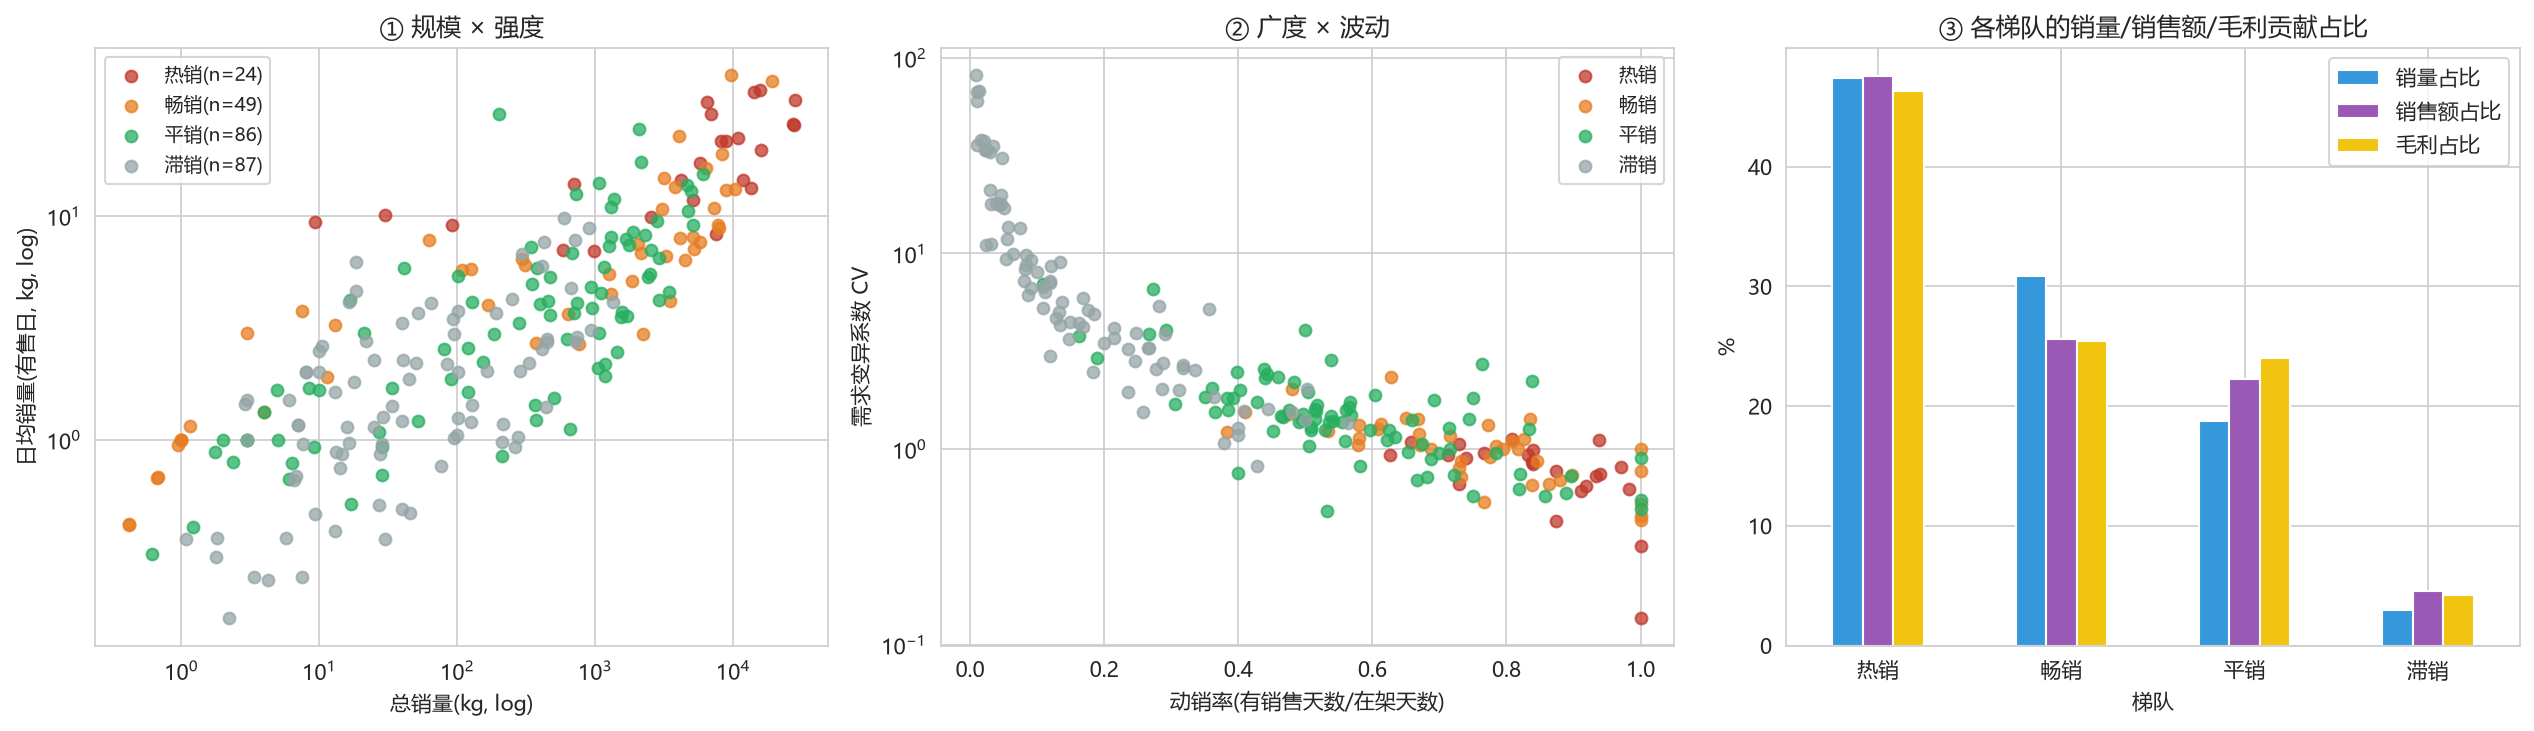
\includegraphics[width=0.92\textwidth]{fig3.png}
\caption{四梯队的规模、强度、广度、波动与贡献对比}
\label{fig:tier4}
\end{figure}

\subsection{Syntetos-Boylan 需求形态分类}

梯队回答给多少货架，形态回答用什么预测模型，两件事分开。采用 Syntetos-Boylan 分类，以平均需求间隔 $\mathrm{ADI}=1.32$ 与变异系数平方 $\mathrm{CV}^2=0.49$ 为界，246 个单品中 Smooth 34 个占 13.8\%，Intermittent 83 个占 33.7\%，Erratic 25 个占 10.2\%，Lumpy 104 个占 42.3\%。也就是说，超过四成的单品需求又稀疏又剧烈，标准的指数平滑在这批单品上没有用武之地。

形态与梯队交叉后对应关系清晰。Lumpy 104 个里 49 个落在滞销梯队、42 个在平销；Smooth 34 个里 27 个在热销或畅销，滞销里一个没有。品类差异更明显，茄类 10 个单品 8 个是 Lumpy，与它夏季集中上市的特征对得上；特别的，花菜类 5 个单品中 2 个 Smooth、3 个 Intermittent，没有 Lumpy，是最适合标准补货模型的品类。形态到模型的映射列成规则：Smooth 走指数平滑加 ROP 定量补货，Intermittent 用 Croston 法或 SBA，Erratic 抬高安全库存，Lumpy 少备勤补、滞销时降价清货，图 \ref{fig:sb} 画出四象限分布。

\begin{figure}[H]
\centering
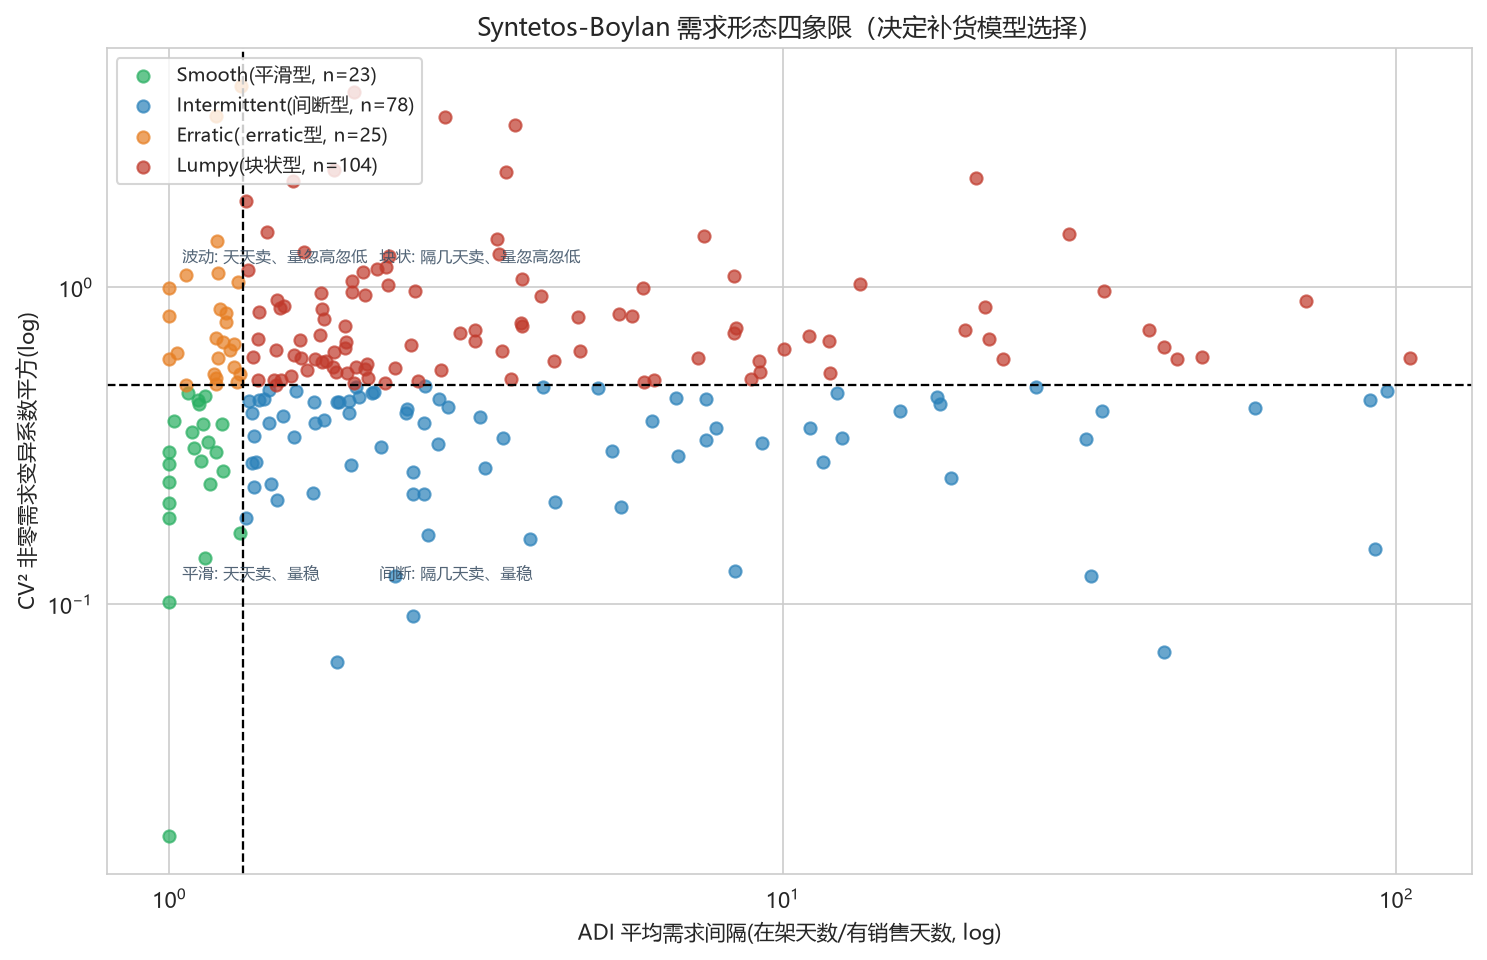
\includegraphics[width=0.86\textwidth]{fig4.png}
\caption{Syntetos-Boylan 需求形态四象限}
\label{fig:sb}
\end{figure}

\subsection{量-利四象限}

四象限的分界线选过两版。先按总销量与总毛利的中位数切，切出来 116 对 116 各半，总销量与总毛利高度同源，中位数切分退化成对角线；改成销量份额与毛利率双轴，以中位数 0.055\% 与 33.15\% 为界，得到明星品 66 个、引流品 57 个、利润品 57 个、问题品 66 个，四个格子终于站得住了。

明星品贡献销量 39.62\%、毛利 39.22\%，毛利率均值 39.64\%，量利双主力。引流品贡献销量 59.22\% 但毛利率只有 26.54\%，芜湖青椒(1)、西兰花、净藕(1) 都在其中，职能是带客流。利润品销量占比仅 0.76\% 而毛利率均值 44.71\%。错位分析还捞出一批隐形利润品，西峡香菇(1) 销量份额 2.53\%、毛利份额 4.89\%；小米椒销量份额 0.31\%、毛利份额 1.44\%；组合椒系列毛利率 81.93\%。反例是大白菜，销量份额 4.07\% 只换来毛利份额 0.93\%，毛利率 24.18\%，典型的引流品，见图 \ref{fig:quadrant}。

\begin{figure}[H]
\centering
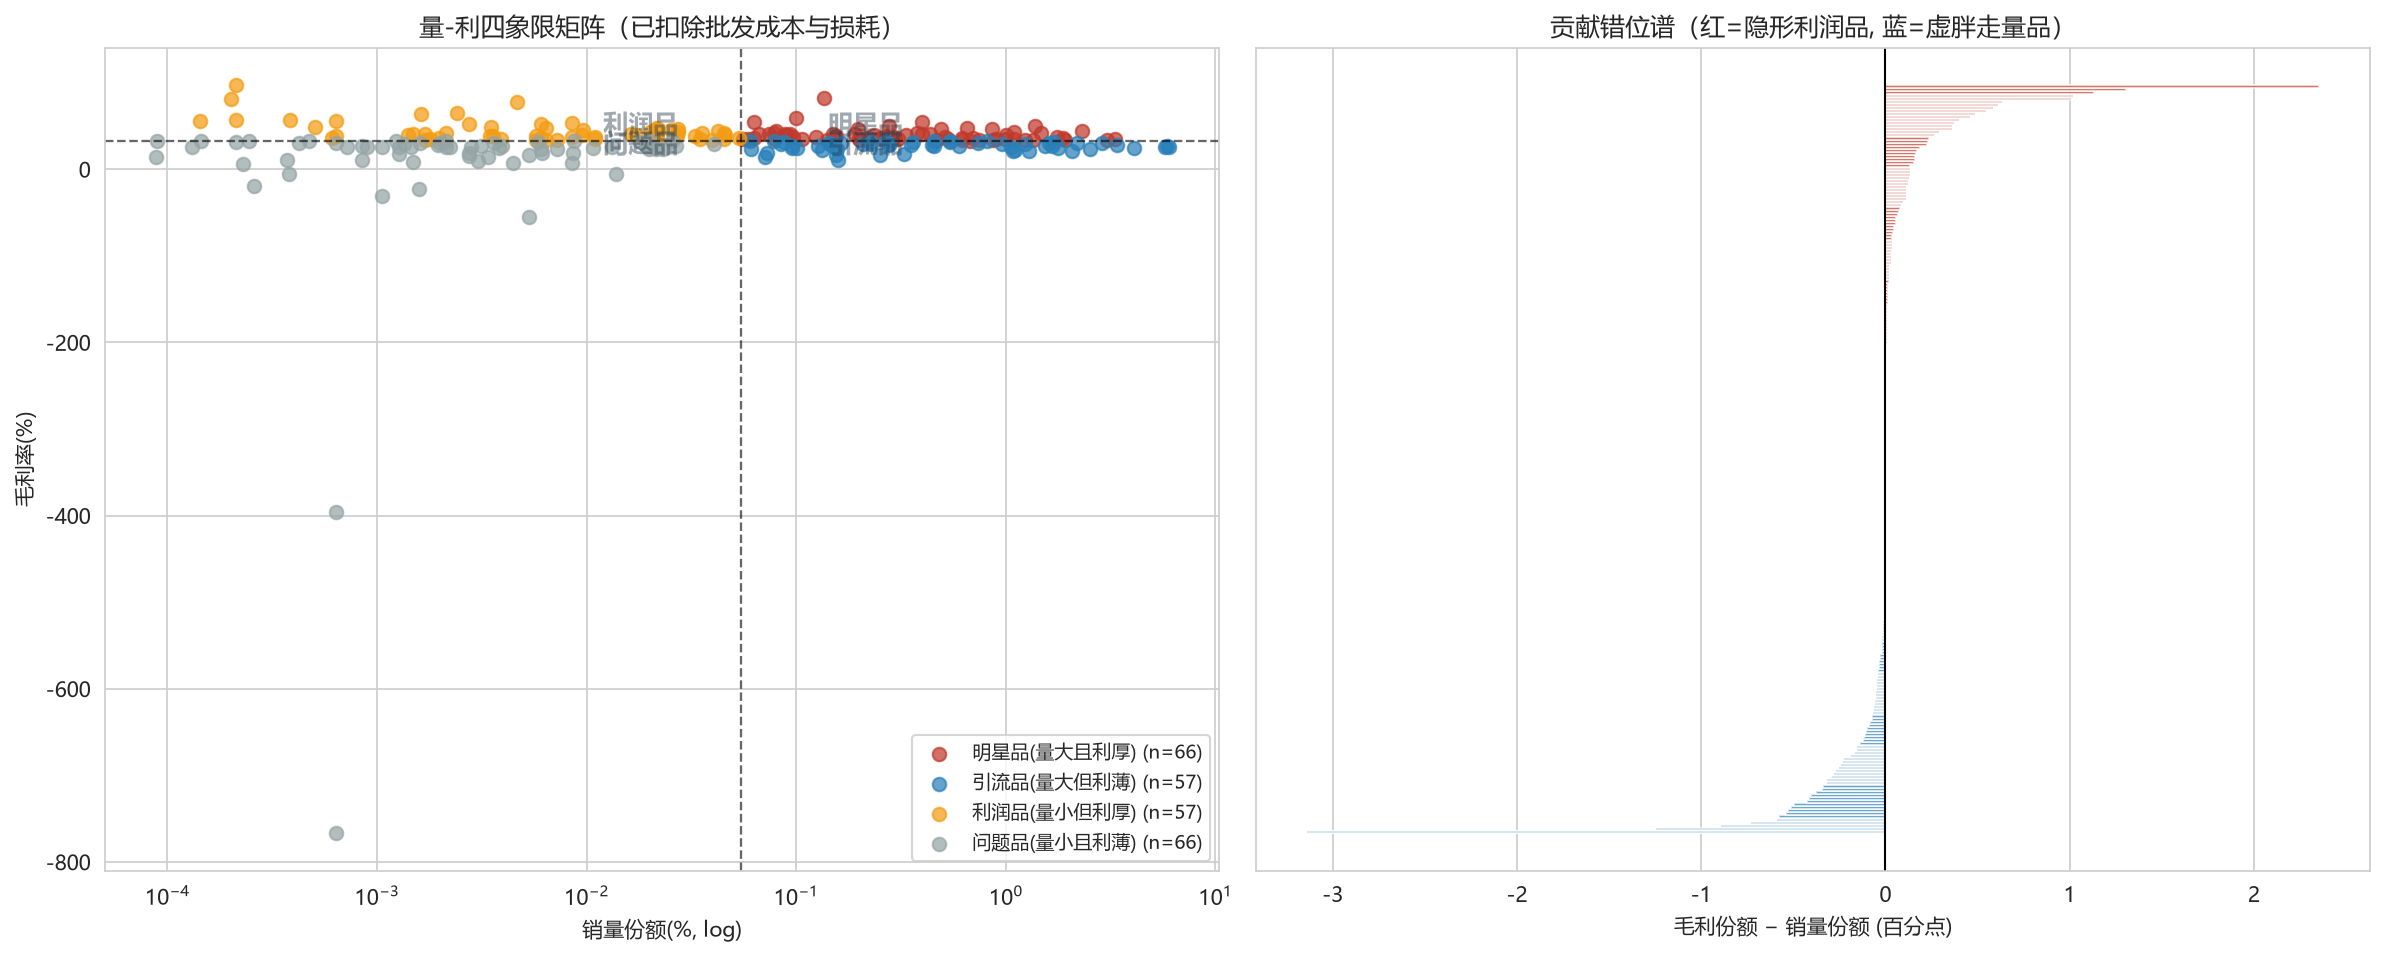
\includegraphics[width=0.9\textwidth]{fig5.png}
\caption{量-利四象限矩阵与代表单品}
\label{fig:quadrant}
\end{figure}

\subsection{季节指纹与生命周期}

月份是环形的，12 月挨着 1 月，直接对月份序号加权平均会把首尾两个月算到年中去。把 12 个月映射到圆周，月份 $m$ 的角度 $\theta_m=2\pi(m-1)/12$，季节重心按加权方向平均求得
\begin{equation}
\bar{\theta}=\operatorname{atan2}\Big(\textstyle\sum_m w_m\sin\theta_m,\ \sum_m w_m\cos\theta_m\Big),
\end{equation}
式中 $w_m$ 为月销量占比。算下来水生根茎类重心 11.2 月、食用菌 12.0 月、辣椒类 1.6 月，三个是冬菜；茄类重心 6.1 月，唯一的夏菜。旺淡倍数按旺季月销量占比除以淡季月销量占比，水生根茎类 6.87 最大，茄类 3.37 次之，食用菌 2.51，辣椒类 1.72 最小。花叶类与辣椒类的一阶圆傅里叶幅度偏小，原因是两者在 1 月与 8 月各有一个峰，双峰相互抵消，重心月份会失真，要配合旺淡倍数一起读。

单品层面做 k-means 聚类，$k$ 取 3、4、5 三档试算。$k=3$ 把冬季峰并进一个簇，$k=4$ 时 31 个冬季峰单品仍混在一团，$k=5$ 才把 1 月峰 19 个与 2 月峰 12 个分开，簇内曲线峰值一致，取 5。结果是弱季节型 178 个、占全部销量 97.7\%；强季节型合计 68 个、销量占比 2.4\%，其中 4 月峰 28 个且花叶类占 18，属春菜，另有 1 月峰 19 个、2 月峰 12 个、7 月峰 9 个。总量的季节性远比单品印象弱，这个现象与 5.8 节的归因结论是一件事的两面。

生命周期按近 180 天是否有销售划分，已退市 110 个、占销量 10.2\%，在架天数均值 183 天；活跃在架 136 个、占销量 89.8\%，在架天数均值 654 天。各品类活跃单品数为花叶类 58、辣椒类 28、食用菌 29、水生根茎类 12、茄类 6、花菜类 3。已退市的单品补不了货，放进任何候选池都没有决策意义，后面问题 3 的选品只在 136 个活跃单品里取。图 \ref{fig:season} 汇总季节与生命周期结果。

\begin{figure}[H]
\centering
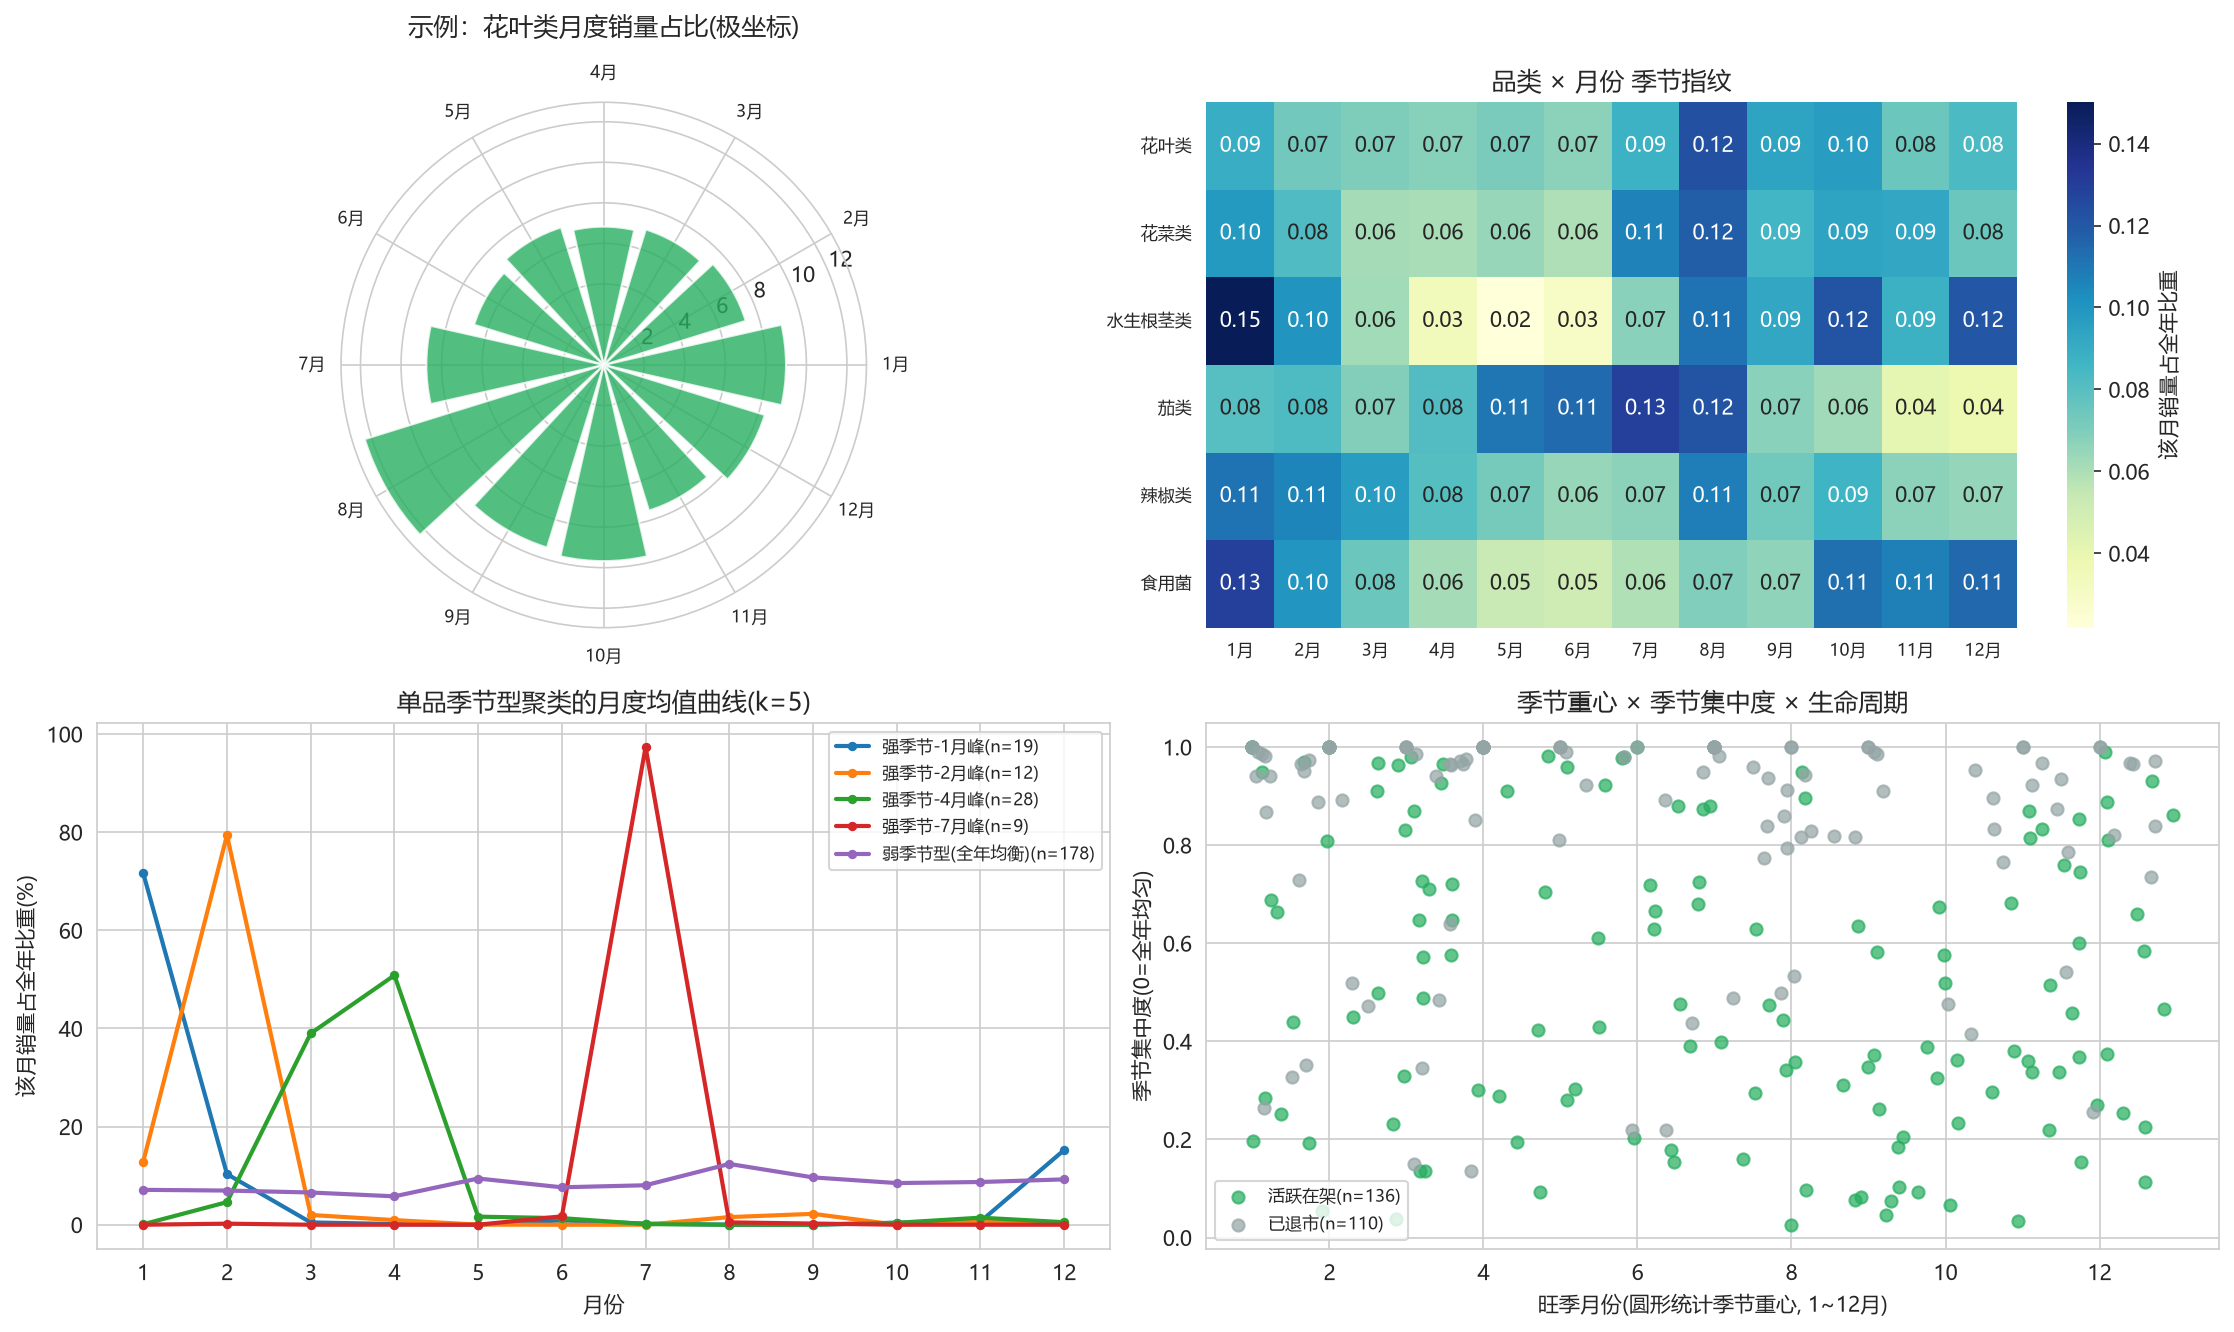
\includegraphics[width=0.95\textwidth]{fig6.png}
\caption{季节指纹聚类与生命周期状态}
\label{fig:season}
\end{figure}

\subsection{品类相关性的三层归因}

把 15 个品类对的日相关系数排出来，茄类的位置扎眼，水生根茎类与茄类只有 0.074，茄类与食用菌 0.120，茄类与花叶类 0.257，表面看茄类接近需求独立。这个结论没有直接采纳，因为低相关有三种来源，月度共同波动、季节指纹相似、日内真实联动，得先分清是哪一种。

两项检验指向第一种来源占主导。日相关对月序列相关做回归，$r=0.981$（$p<0.0001$），品类对的日相关几乎完全由月度层面的共同波动决定；日相关对季节指纹相似的 $r=0.822$（$p=0.0002$）。归因实验是去季节，把每日销量除以本品类月度季节指数再算相关，15 个品类对的平均相关从 0.473 升到 0.523，茄类与食用菌从 0.120 升到 0.393，水生根茎类与茄类从 0.074 升到 0.303，花叶类与茄类从 0.257 升到 0.398，见图 \ref{fig:attrib}。

机理在季节相位。茄类旺季 7 月占其销量 12.9\%，淡季 12 月只有 3.8\%；冬菜的旺季在 12 月至次年 1 月。夏菜与冬菜的销量曲线接近反相，季节项贡献了负相关，把同一天里真实的日内联动盖住了，去季节后恢复的 0.30$\sim$0.40 就是被盖住的部分。据此修正初步判断，茄类并非需求独立，低相关是季节相位制造的假象。这条结论直接进问题 2 的建模清单，品类联合补货模型要保留联动项，同时显式引入各品类的季节相位。

\begin{figure}[H]
\centering
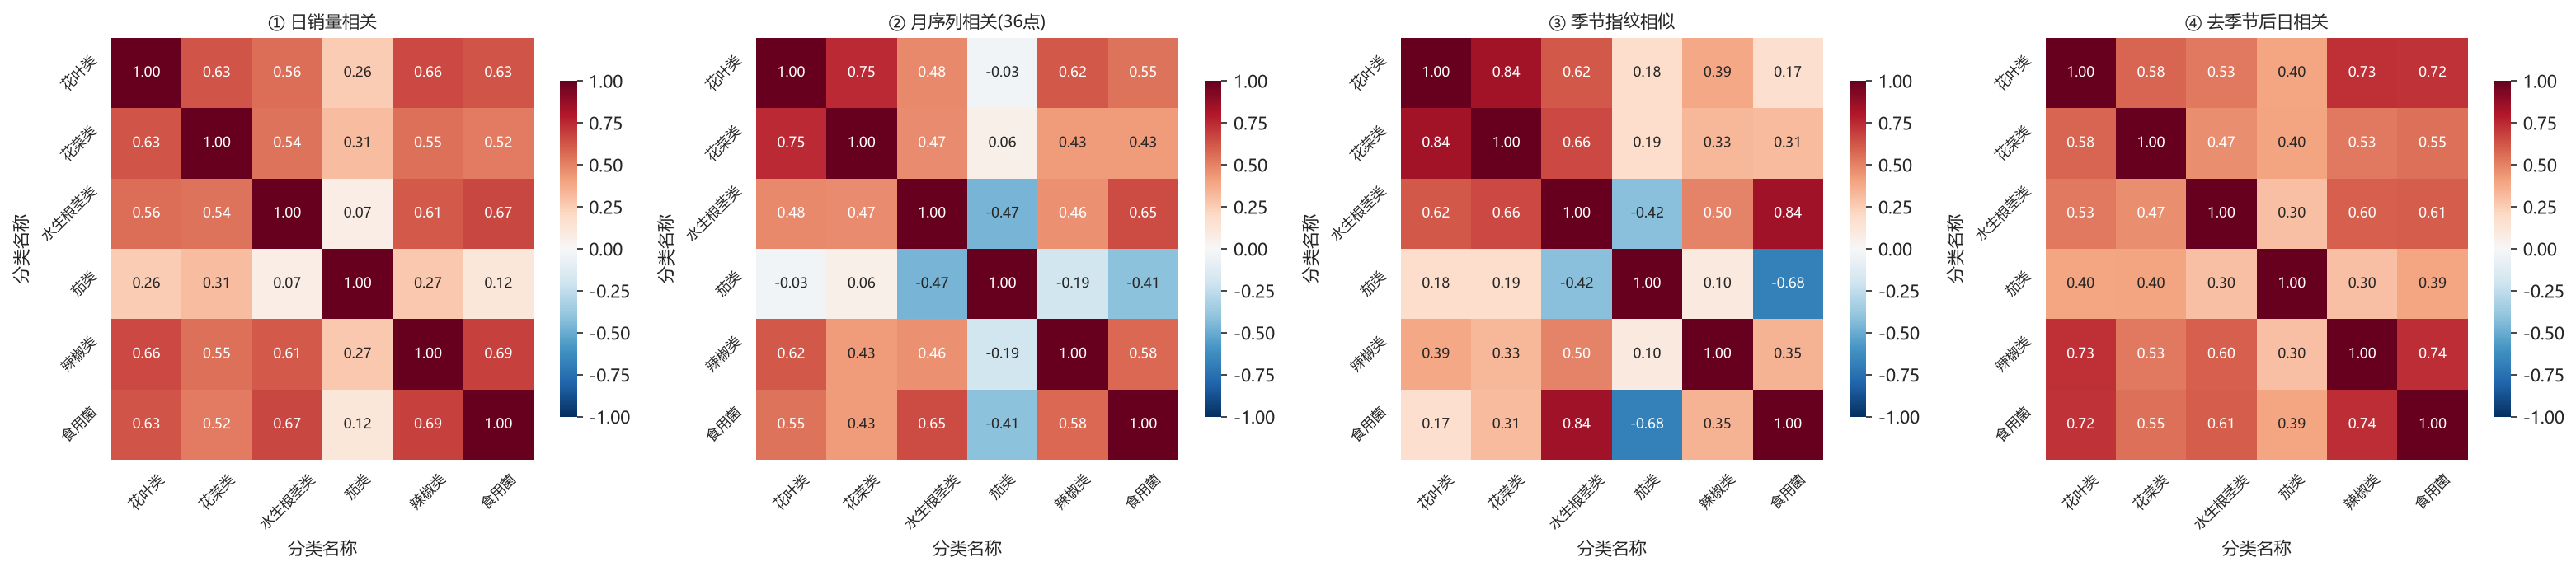
\includegraphics[width=0.95\textwidth]{fig7.png}
\caption{品类相关性的三层归因：日相关、月序列相关与季节指纹相似}
\label{fig:attrib}
\end{figure}

\subsection{共现网络、互信息与替代关系}

单品之间的关系换一条通道看，不看销量共变，看同日共现。共现强度用 lift 而不用支持度，支持度反映单品自身热度，热门单品与谁共现都偏高；lift 把热度本身剔除，定义为实际共现天数与独立假设下期望共现天数之比
\begin{equation}
\mathrm{lift}_{AB}=\frac{c_{AB}}{N_A N_B/N_d},
\end{equation}
式中 $c_{AB}$ 为同日共现天数，$N_A$、$N_B$ 为各自出现天数，$N_d$ 为统计天数。流水按天二值化后 246 个单品在 1,085 天内的整体购买率 0.175，共现天数范围 0$\sim$1,076 天。保留出现不少于 60 天的 132 个单品，以共现不少于 40 天且 lift 不低于 1.35 建边，得到 122 个节点、1,990 条边的网络，Louvain 社团划分给出 3 个社团，模块度 $Q=0.3983$，高于 0.3 的经验显著线，图 \ref{fig:network} 画出网络与社团。

三个社团规模 59、52、11 个单品，主导品类都是花叶类，分别 24、16、4 个，但每个社团横跨 4$\sim$6 个品类，社团 1 的代表单品为田七、荸荠、大龙茄子、金针菇(1)，社团 2 的代表为青杭椒(份)、龙牙菜、上海青(份)、菜心(份)。共现结构由购物篮的组合方式决定，与品类归属关系不大，做关联陈列按社团取品比按品类取品更有效。

Pearson 相关只度量销量数值的线性共变，补一个归一化互信息，把两单品是否同日出现的依赖强度压到 0$\sim$1 区间，
\begin{equation}
\mathrm{NMI}(A,B)=\frac{I(A;B)}{\sqrt{H(A)H(B)}},
\end{equation}
式中 $I(A;B)$ 为互信息，$H$ 为信息熵。Top40 单品上 NMI 与 Pearson 的 Spearman $\rho$ 为 $-0.016$（$p=0.66$），两者近乎正交，回答的是两个不同的问题。两个方向的案例都有，净藕(1) 与茼蒿 Pearson 高达 0.529 而 NMI 只有 0.003，是同季供应造成的伪相关；云南油麦菜与云南油麦菜(份) Pearson 为 $-0.440$ 而 NMI 有 0.406，这种同日出现而此消彼长的依赖线性方法会漏掉。

替代关系在同款不同规格单品内部最清晰。36 组同款不同规格的对子里 lift 小于 1 的有 23 组，共售日条件相关为负的有 19 组，两者倾向于不在同一天出现。散装与份装互斥，云南生菜单装对份装 lift 0.452、全样本相关 $-0.836$，小米椒 0.255，奶白菜 0.338，菜心 0.388。菌菇的盒装与袋装正好相反，杏鲍菇(1) 对杏鲍菇(袋) 共现 297 天、lift 2.180，金针菇(1) 对金针菇(袋)(1) lift 2.402，海鲜菇(2) 对海鲜菇(袋)(3) lift 4.521。两类包装是两门生意，前者同一批客人二选一，后者面向不同采购用途、经常一起买。定价上的含义分开处理，散装与份装要拉开价差避免左右互搏，菌菇不同规格可做组合促销。

\begin{figure}[H]
\centering
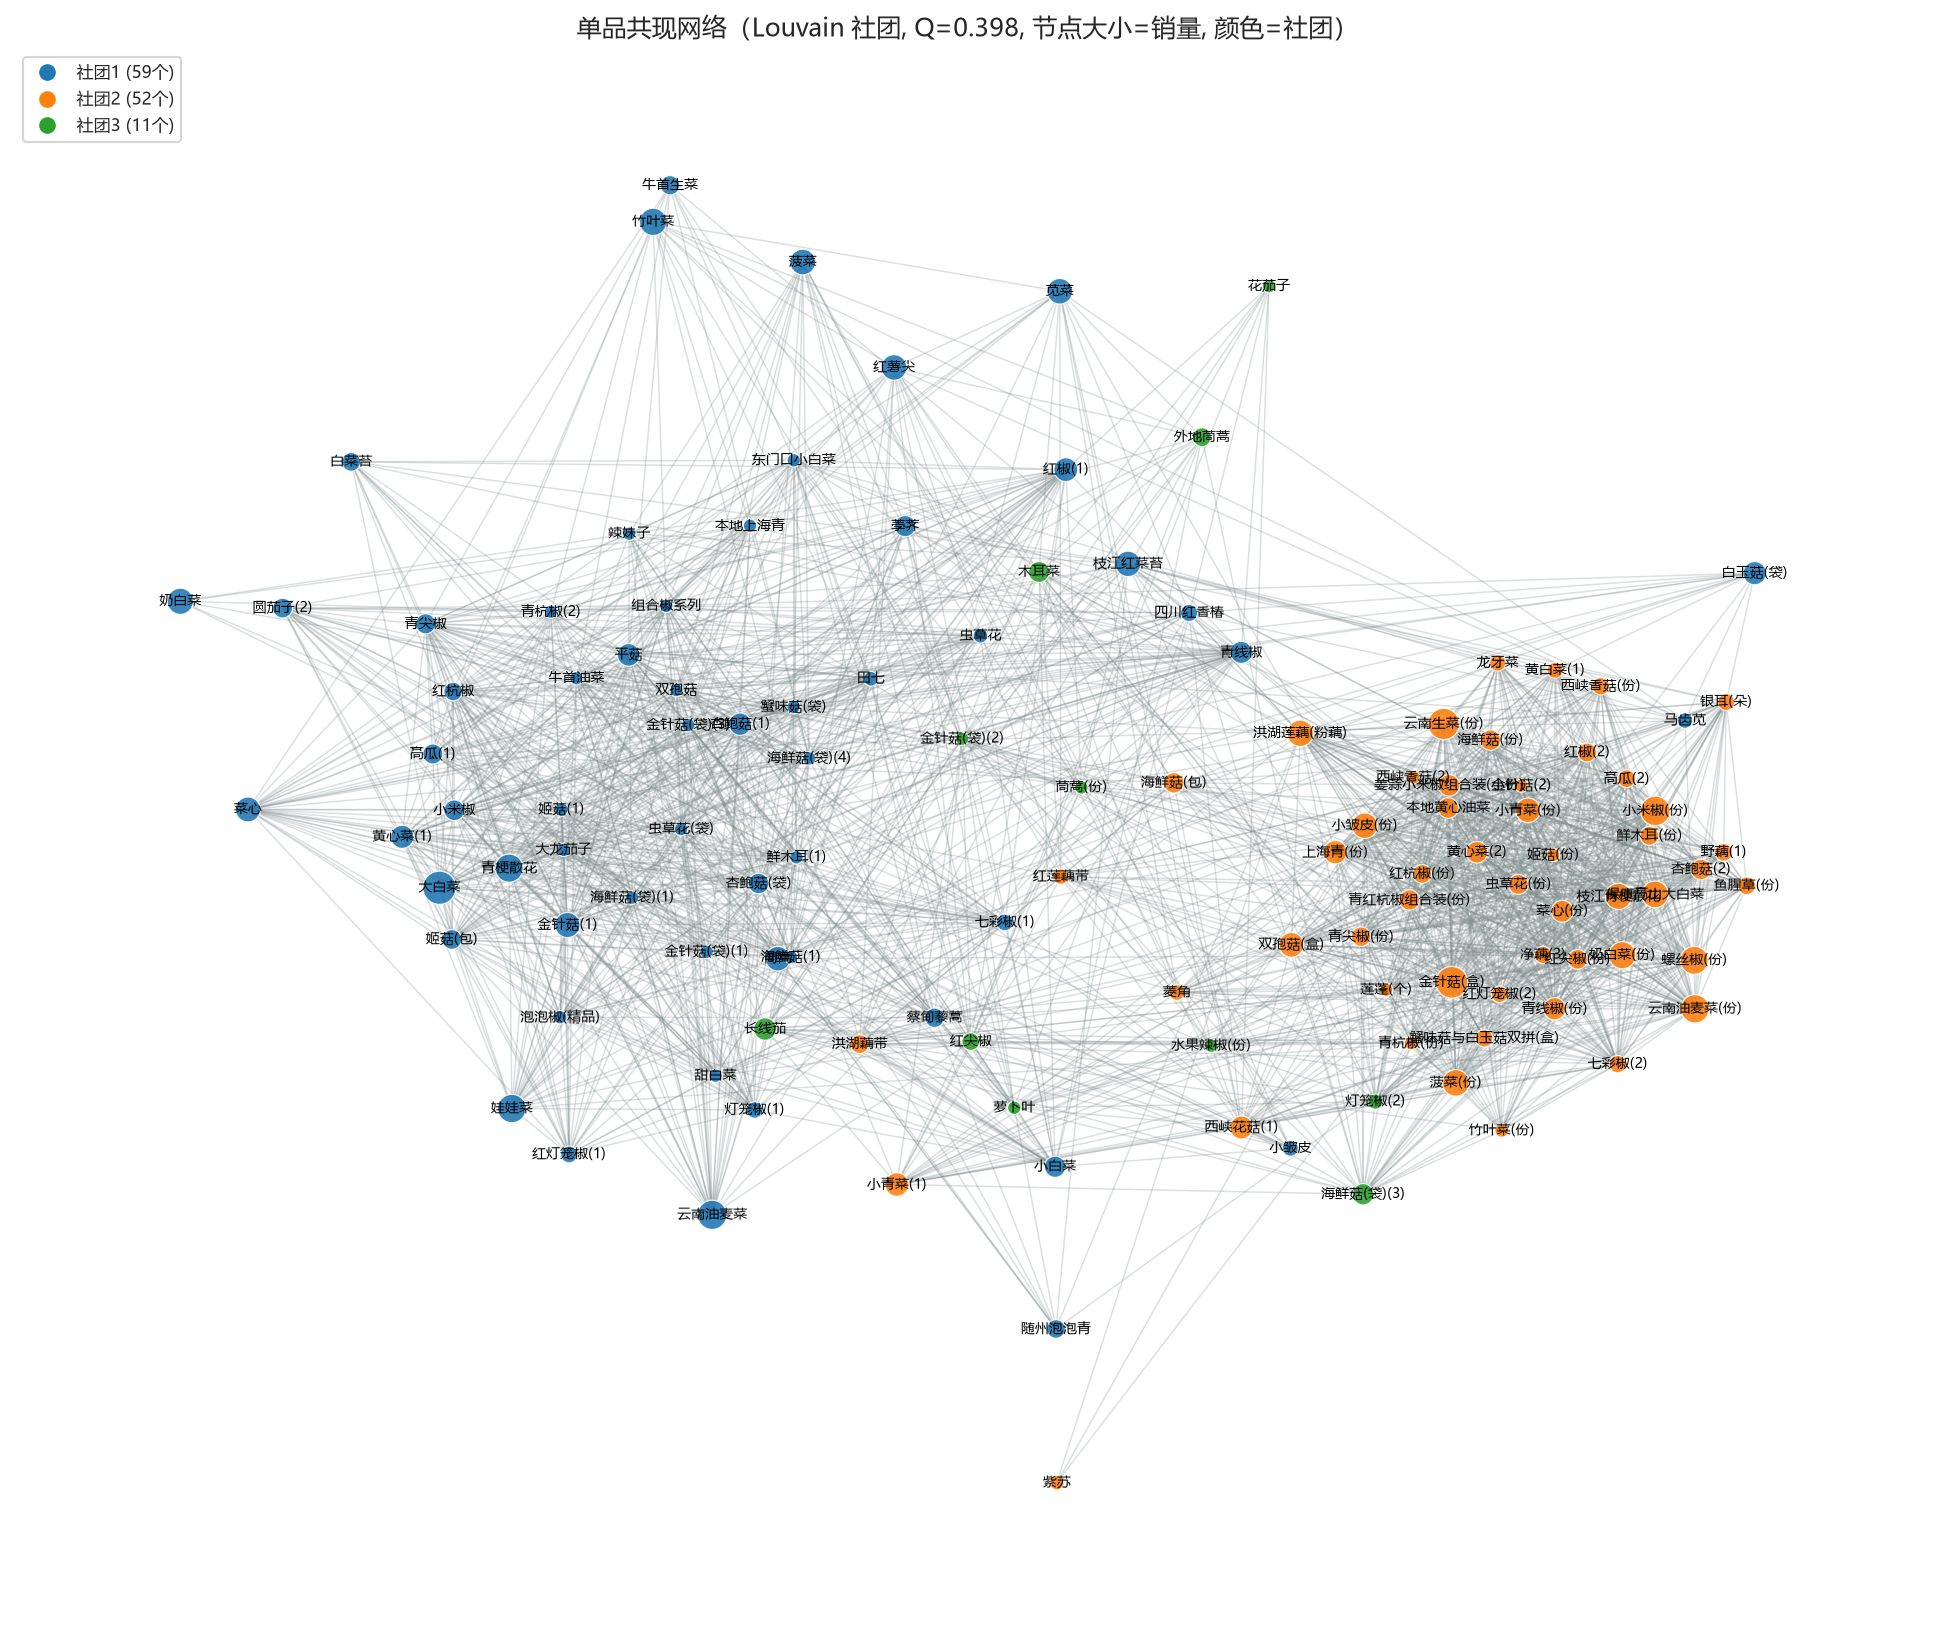
\includegraphics[width=0.9\textwidth]{fig8.png}
\caption{单品共现网络与 Louvain 社团}
\label{fig:network}
\end{figure}

\subsection{货位效率与推荐选品}

评价一个单品值不值得占货位，用日毛利产出，定义为单位毛利乘以在架日销量；另设卖完一货位天数等于 2.5 除以日均销量，对应题目问题 3 的最小陈列量 2.5 kg，
\begin{equation}
E=m\,\bar q,\qquad T=\frac{2.5}{\bar q},
\end{equation}
式中 $\bar q$ 为在架日销量。只按单位毛利排序会误导，小米椒单位毛利 9.99 元/kg，日均只卖 1.40 kg，日毛利产出 13.95 元/天；大白菜单位毛利 0.49 元/kg，日均 19.17 kg，日毛利产出 9.36 元/天。单位毛利差 20.5 倍，同一块 2.5 kg 货位的日毛利产出只差 1.5 倍，这笔账是算得清的。

候选池 136 个单品中，日毛利产出前五为西兰花 65.56 元/天、芜湖青椒(1) 51.57 元/天、西峡香菇(1) 49.71 元/天、净藕(1) 49.25 元/天、小米椒(份) 43.79 元/天；垫底的是洪山菜薹珍品手提袋 $-176.00$ 元/天与洪山菜薹莲藕拼装礼盒 $-28.79$ 元/天，这两个亏损品每在架一天都在净亏。分梯队看，热销 34.12、平销 6.15、畅销 4.12、滞销 1.16 元/天，畅销反而低于平销，原因是畅销梯队里有洪山菜薹两个深亏品拉低了均值，梯队标签不能替代效率核算。

以日毛利产出为主序贪心选取 30 个单品并强制覆盖 6 品类，得到推荐池，花叶类 11 个、辣椒类 7 个、食用菌 6 个、花菜类 2 个、水生根茎类 2 个、茄类 2 个；梯队构成热销 18、畅销 6、平销 6；需求形态 Smooth 5、Erratic 10、Intermittent 7、Lumpy 8。该池覆盖门店总销量的 60.6\% 与总毛利的 63.3\%，池内卖完一货位最慢的是小米椒，也只要 1.79 天，可直接作为问题 3 的初始解。题目问题 3 要求从 2023 年 6 月 24 日至 30 日的可售品种中选品，本文候选池取近 180 天有销售的 136 个活跃单品，比题目窗口更宽，是为了给初始解留出替换余地，正式求解时按题意收紧到该周在售品种即可。图 \ref{fig:slot} 汇总货位效率与选品结果。

\begin{figure}[H]
\centering
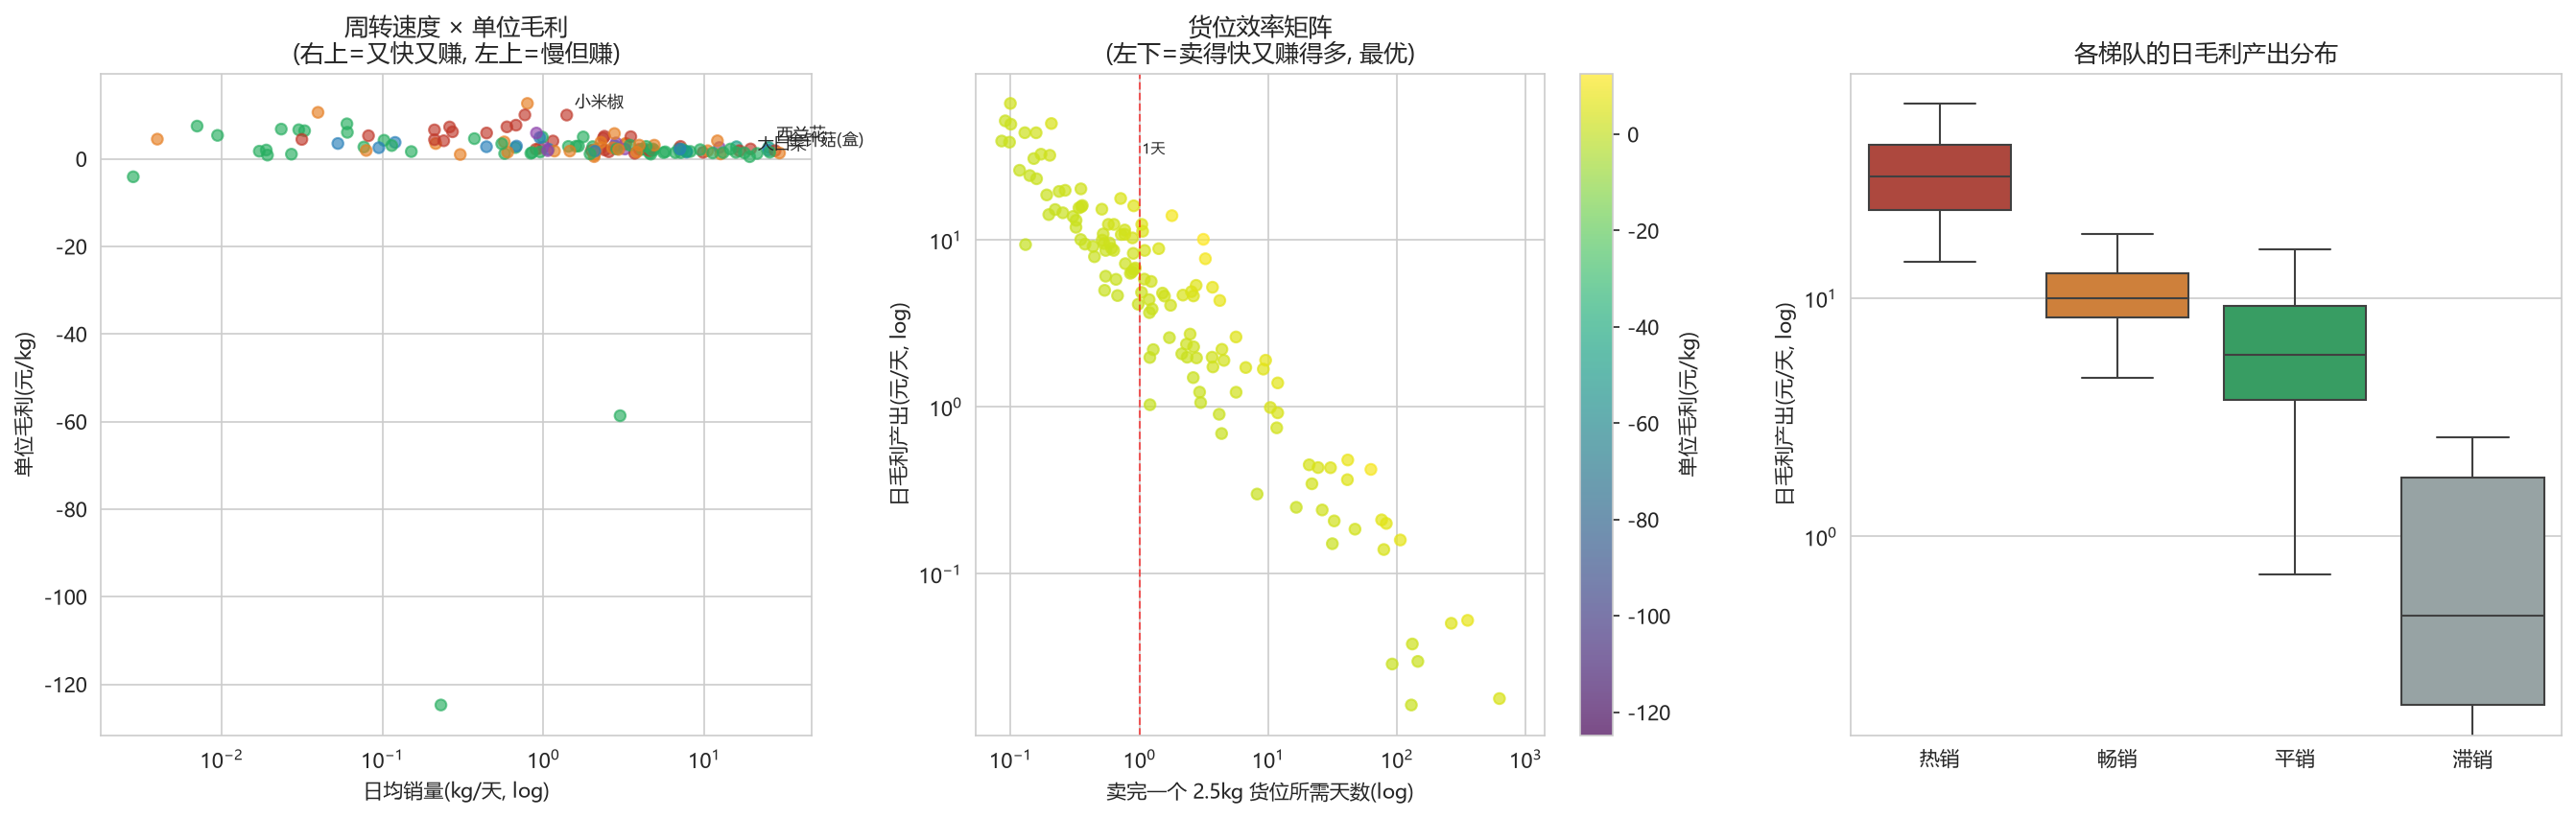
\includegraphics[width=0.95\textwidth]{fig9.png}
\caption{货位效率排序与 30 单品推荐池构成}
\label{fig:slot}
\end{figure}

\subsection{问题 1 结论}

问题 1 的答案可以收成七条。

\begin{enumerate}
  \item 分布高度长尾。28 个 A 类单品占单品数 11.4\%，贡献销售额 69.27\%；183 个 C 类单品合计只贡献 10.19\%；24 个热销单品贡献 47.42\% 销量与 46.35\% 毛利。
  \item 均价低不等于不赚钱。花叶类相对价格指数 0.76 为六品类最低，毛利率 31.18\% 仍居第一梯队；大白菜以 4.07\% 的销量份额只换回 0.93\% 的毛利份额，毛利由损耗率与周转共同决定。
  \item 稳定比规模更稀缺。熵权法给广度的权重 0.2928 为四维最高；34 个 Smooth 单品动销率 0.942，是唯一适合标准预测补货模型的一批。
  \item 季节相位决定品类关系的表象。茄类是唯一夏菜，重心 6.1 月、旺淡倍数 3.37，与三个冬菜的表面相关仅 0.074$\sim$0.257，去季节后恢复至 0.30$\sim$0.40，品类联动真实存在。
  \item 共现结构由购物篮组合决定，与品类归属关系不大。1,990 条边的网络分成 3 个跨品类社团，模块度 0.3983，关联陈列应按社团取品。
  \item 同款不同规格是两类生意。36 组对子里 23 组散装对份装 lift 小于 1，为替代关系；菌菇盒装与袋装 lift 2.18$\sim$4.52，为互补关系，定价与促销策略应分开。
  \item 货位按日毛利产出分配。30 单品推荐池覆盖销量 60.6\%、毛利 63.3\%，货位周转最慢 1.79 天；洪山菜薹两个亏损品日亏 28.79$\sim$176.00 元，应首先移出货位。
\end{enumerate}

% =====================================================================
\section{问题2模型的建立与求解}
% ===== 问题 2（留空，由负责该问的队友补写）=====
% TODO 模型：各品类销售总量与成本加成定价的关系
% TODO 求解：2023 年 7 月 1--7 日各品类日补货总量与定价策略
% 可用起点：5.8 节结论（品类联合模型保留联动项，并显式引入季节相位）
%          表 1 的品类毛利结构与 5.7 节的季节重心、旺淡倍数

\section{问题3模型的建立与求解}
% ===== 问题 3（留空，由负责该问的队友补写）=====
% TODO 模型：27~33 个可售单品的约束优化（最小陈列量 2.5 kg）
% TODO 求解：基于 2023 年 6 月 24--30 日可售品种的 7 月 1 日单品补货量与定价
% 可用起点：5.10 节的 30 单品推荐池（覆盖销量 60.6%、毛利 63.3%）作初始解，
%          候选池按题意收紧到 6 月 24--30 日在售品种；货位周转天数 T 见式 (7)

\section{问题4模型的建立与求解}
% ===== 问题 4（留空，由负责该问的队友补写）=====
% TODO 方向参考：小票级数据（补同篮共现）、到货损耗记录（补成本口径）、
%               竞品价格与客流数据（补需求弹性）——仅作提示，内容自定

\section{模型的评价与推广}

\subsection{优点}

成本修正改变了结论而不只是精度。修正前毛利账整体偏高 7.7\%$\sim$16.5\%，8 个亏损单品与两个深亏礼盒全部隐身，四象限的利润品名单会是另一份名单。

分层的有效性可由数据自证。TOPSIS 得分与总销量的 Spearman $\rho=0.527$、与动销率 $\rho=0.884$，分层引入了规模之外的信息量；ABC-XYZ 的 CZ 格 61 个单品仅贡献 1.77\% 销售额，区分度落在销售额上而不只在计数上。

归因避免了两个方向的误判。若无三层归因，茄类会被当成需求独立品剔出联动模型，问题 2 的品类联动项就丢了；若无 NMI 对照，云南油麦菜散装与份装的此消彼长（Pearson $-0.440$、NMI 0.406）会被漏掉。

\subsection{缺点与适用边界}

批发价填充的误差无法从数据内部检验。缺失率 79.6\%，填充用的是单品中位数，若某单品价格在样本期内有趋势性上行，有效成本会被系统性低估，此偏差没有独立的价格源可对照。改进方向是引入时间加权均价，代价是早期样本进一步变薄。

建边阈值为经验值。保留阈值 60 天、建边阈值 40 天与 lift 1.35 均未做灵敏度扫描，社团结构 $Q=0.3983$ 对阈值的稳健性未知。改进方向是对三个阈值各做 $\pm 20\%$ 扫描并复算模块度，代价是计算量与报告篇幅。

共现以天为粒度，丢失同篮信息。附件 2 只有天粒度流水，无法区分一次购物篮内的组合与同日两笔独立购买，NMI 与 lift 度量的都是同日出现，这层损失在本数据下无法弥补。

归因结论的适用边界在相位差上。旺淡倍数很低的品类（本文最平缓的辣椒类只有 1.72）季节项本身弱，去季节处理带来的恢复量有限，此时表面相关已接近真实联动；旺淡倍数在 3 以上的品类对（水生根茎类 6.87、茄类 3.37）才是归因框架收益最大的场景。

\subsection{推广}

全息画像与四套分层的组合不依赖蔬菜属性，换成日配、烘焙等短保品类同样适用。三层归因的框架对任何存在强季节相位的时间序列共变分析都有效，先拆相位再看联动，避免把季节错峰当成需求独立。

% ---------------------- AI 工具使用声明 ----------------------
\section*{AI 工具使用声明}
本小组在清洗脚本编写、图表绘制与初稿撰写环节使用了 AI 工具辅助，使用范围与交互记录（工具版本、使用环节、关键提示词）由本小组留存备查。全部数值逐项核对自脚本运行日志，模型选型的决策记录与最终结论由小组成员复核认定。
% 请按小组实际情况修改本节表述，竞赛要求支撑材料中另附 AI 工具使用详情。

% ---------------------- 参考文献 ----------------------
\section*{参考文献}
% TODO：如正文有引用在此补充条目，严禁编造文献。

% ---------------------- 附录 ----------------------
\appendix

\section{核心代码节选}

熵权-TOPSIS 的核心实现如下，全部代码见仓库 问题1-SKU全息画像与关联分析/code/ 目录（00 数据清洗、04 画像与分层、05 归因与网络）。

\begin{verbatim}
def entropy_weight_topsis(X):
    Z = (X - X.min()) / (X.max() - X.min()); Z = Z.clip(lower=1e-6)
    P = Z.div(Z.sum(axis=0), axis=1); k = 1.0/np.log(len(Z))
    E = -k*(P*np.log(P)).sum(axis=0); d = 1.0-E; W = d/d.sum()
    V = Z*W; vpos, vneg = V.max(), V.min()
    Dp = np.sqrt(((V-vpos)**2).sum(axis=1)); Dn = np.sqrt(((V-vneg)**2).sum(axis=1))
    return Dn/(Dp+Dn), W
\end{verbatim}

% 完整代码清单如需排入附录，取消下行注释并按实际路径修改
% （需 listings 宏包，XeLaTeX 下中文注释建议改用 minted 或临时删除注释）：
% \lstinputlisting[language=Python]{问题1-SKU全息画像与关联分析/code/04_问题1_升级_SKU全息画像与分层.py}
% \lstinputlisting[language=Python]{问题1-SKU全息画像与关联分析/code/05_问题1_升级_相关归因与共现网络.py}

\end{document}
